\documentclass[UTF-8]{article}
\usepackage{amsmath}
\usepackage{amssymb}
\usepackage{float}
\usepackage{graphicx}
\usepackage{epstopdf}
\usepackage{inputenc}
\usepackage{geometry}
\usepackage{pgfplots} 
\usepackage{listings}
\usepackage{enumitem}
\usepackage{lipsum}  
\usepackage{color}

\usepackage[colorlinks=true, urlcolor=blue, linkcolor=blue]{hyperref}
\geometry{left=2.5cm,right=2.5cm,top=2.5cm,bottom=2.5cm}

\definecolor{codegreen}{rgb}{0,0.6,0}
\definecolor{codegray}{rgb}{0.2,0.2,0.2}
\definecolor{codepurple}{rgb}{0.58,0,0.82}
\definecolor{backcolour}{rgb}{0.95,0.95,0.952}

\lstdefinestyle{mystyle}{
	backgroundcolor=\color{backcolour},   
	commentstyle=\color{codegreen},
	keywordstyle=\color{blue},
	numberstyle=\tiny\color{codegray},
	stringstyle=\color{codepurple},
	basicstyle=\ttfamily\footnotesize,
	breakatwhitespace=false,         
	breaklines=true,                 
	captionpos=b,                    
	keepspaces=true,                 
	numbers=left,                    
	numbersep=5pt,                  
	showspaces=false,                
	showstringspaces=false,
	showtabs=false,                  
	tabsize=2,
	 linewidth=1.185\linewidth,
	 resetmargins=true,
	 xleftmargin=-1cm,
	 xrightmargin=0.085\textwidth,
	prebreak = \raisebox{0ex}[0ex][0ex]{\ensuremath{\hookleftarrow}}
}

\lstset{style=mystyle}
\pgfplotsset{compat=1.18}
\parindent 0cm

\title{High Performance Computing Proseminar 2024 \\
    \large Assignment 3} %exchange for assignment number

\author{Stefan Wagner \& Sebastian Bergner\\Team: Planning Desaster}
\begin{document}
    
    \maketitle
    
    The goal of this assignment is to improve the 2D heat stencil application.
    
    \section*{Exercise 1}
    This exercises consists in improving the 2D heat stencil application, fixing any existing bugs and/or improving its performance.
    \\
    \textbf{Tasks}
    \begin{itemize}
    	\item If you need to fix errors, run through the usual debugging workflow detailed in the lecture on debugging:
    	\begin{enumerate}[label=\roman*]
    		\item enable compiler warnings
    		\item check with sanitizers
    		\item run with a debugging tool of your choice (a working installation of MUST for debugging MPI applications on LCC3 is provided in \verb|/scratch/c703429/software/must-1.9.1|)
    		\\
    		\\
    		\textbf{We started using a functional version, thus omitting this first task.}
    	\end{enumerate}
    	\item If you are looking to improve performance, do a detailed performance analysis. Use either tools discussed in the lecture (perf, gprof, gperftools, etc.) or any tools you deem fit for generating a performance profile. Provide a report that discusses the most expensive source code locations ("hot spots") along with explaining why they are expensive and how to possibly improve on that. Compare blocking and non-blocking if possible, as well as 1D and 2D if you get bored otherwise.
    	
    	
    	We did a bunch of testing, first we analyzed the performance of builds compiled with \verb|-O0| using gprof and perf, but we discussed and found it would make sense to measure the performance (or rather behavior) of the program when compiled with \verb|-O3|.
    	
\subsection*{Gprof output sequential -O3}

The results of the sequential analysis are not helping much, besides finding out that most of the time is spent in the main function (which most probably is the computation itself).
\begin{lstlisting}
Each sample counts as 0.01 seconds.
cumulative   self              self     total           
time   seconds   seconds    calls  Ts/call  Ts/call  name    
97.64     27.73    27.73                             main
0.00      27.73     0.00        6     0.00     0.00  print_temperature
0.00      27.73     0.00        2     0.00     0.00  create_matrix
0.00      27.73     0.00        1     0.00     0.00  data_to_csv	
\end{lstlisting}



\subsection*{Gprof output parallel blocking -O3}

For the blocking program we can observe that there are some more functions. \verb|calc_index_supermatrix| is being called quite often, but has low impact ($< 1 \%$).
\begin{lstlisting}
Each sample counts as 0.01 seconds.
%   cumulative   self              self     total           
time   seconds   seconds    calls  Ts/call  Ts/call  name    
100.24      7.16     7.16                             main
0.00        7.16     0.00   737280     0.00     0.00  calc_index_supermatrix
0.00        7.16     0.00        8     0.00     0.00  create_matrix
0.00        7.16     0.00        8     0.00     0.00  create_vector
0.00        7.16     0.00        6     0.00     0.00  print_temperature
0.00        7.16     0.00        5     0.00     0.00  gather_data_from_submatrices
0.00        7.16     0.00        1     0.00     0.00  calc_rank_factors
0.00        7.16     0.00        1     0.00     0.00  data_to_csv
\end{lstlisting}


\subsection*{Gprof output parallel non-blocking -O3}

For the first time, we can observe a drastic difference. The non-blocking program has been structured differently, moving the computation inside a separate function. Thus making the computation more distinguishable. But identifying "hot-spots" besides the computation remains hard (if not impossible).
\begin{lstlisting}
Each sample counts as 0.01 seconds.
%   cumulative   self              self     total           
time   seconds   seconds    calls  ms/call  ms/call  name    
99.50      6.77     6.77   115200     0.06     0.06  propagate_heat
0.44       6.80     0.03                             main
0.15       6.81     0.01        6     1.67     1.67  print_temperature
0.15       6.82     0.01        1    10.02    10.02  data_to_csv
0.00       6.82     0.00   737280     0.00     0.00  calc_index_supermatrix
0.00       6.82     0.00        8     0.00     0.00  create_matrix
0.00       6.82     0.00        8     0.00     0.00  create_vector
0.00       6.82     0.00        5     0.00     0.00  gather_data_from_submatrices
0.00       6.82     0.00        1     0.00     0.00  calc_rank_factors
\end{lstlisting}


So looking at the above outputs, we cannot conclude much more than that the computation most probably takes up the majority ($\ge 99 \%$) of the execution time.


\subsection*{Perf output -O0}
\begin{table}[H]
\tiny
\centering
\begin{tabular}{|l|r|r|r|r|r|r|r|}
\hline
Program & L1d load misses & L1d loads & LLC load misses & LLC loads & Time (s) & User time (s) & Sys time (s) \\ \hline
2D\_seq\_debug 384 & 1,420,684,620 & 271,673,069,550 & 10,609 & 27,885,185 & 100.128659 & 99.884303 & 0.002983 \\ \hline
2D\_par\_blocking\_debug 384 & 263,918,449 & 196,663,072,308 & 130,081 & 25,743,849 & 97.633189 & 97.267849 & 0.051793 \\ \hline
2D\_par\_non\_blocking\_debug 384 & 276,756,820 & 197,688,716,869 & 117,548 & 28,575,851 & 96.544740 & 96.110856 & 0.067598 \\ \hline
\end{tabular}
\caption{Perf measurement -O0}
\label{table:perf1}
\end{table}



\subsection*{Perf output -O3}
\begin{table}[H]
\tiny
\centering
\begin{tabular}{|l|r|r|r|r|r|r|r|}
\hline
Program & L1d load misses & L1d loads & LLC load misses & LLC loads & Time (s) & User time (s) & Sys time (s) \\ \hline
2D\_seq\_debug 384 & 1,418,812,102 & 28,372,084,936 & 3,399 & 27,291,708 & 22.882091899 & 22.806702000 & 0.002974000 \\ \hline
2D\_par\_blocking\_debug 384 & 261,226,191 & 8,665,614,974 & 84,869 & 16,154,820 & 7.556716632 & 7.374099000 & 0.038544000 \\ \hline
2D\_par\_non\_blocking\_debug 384 & 275,399,148 & 8,702,055,510 & 85,964 & 18,602,539 & 6.374551468 & 6.190521000 & 0.043667000 \\ \hline
\end{tabular}
\caption{Perf measurement -O3}
\label{table:performance_metrics}
\end{table}

    	
TODO description HIGH L1 load misses 
    	
    	
    	
    	
    	
    	
    	
    	
    	
    	
    	
    	
    	
    	
    	
    	
    	\item Improve your stencil application using the instructions above. When you do, document the improvement you managed to achieve. If you don't, argue why you failed or think you hit the limit.
    	
    	We tried multiple approaches to improve our benchmark performance. At first we tried changing the distribution pattern of the grid to one where ranks obtain multiple "full" rows. We did this, despite having an "optimal" implementation (of the access pattern) because we couldn't measure wall times resembling this.
    	
    	Using this new blocking (or \textbf{slicing} that's how we called it) approach we would avoid many cache misses, otherwise introduced by copying into a send and receive buffer each iteration (which should occur quite often in the left and right buffers).
    	
    	\begin{lstlisting}[language=c]
for (int i = 0; i < cols_per_rank; i++){
	send_up_temps[i] = A[calc_index(0, i, cols_per_rank)];
}
for (int i = 0; i < cols_per_rank; i++){
	send_down_temps[i] = A[calc_index(rows_per_rank-1, i, cols_per_rank)];
}
for (int i = 0; i < rows_per_rank; i++){
	send_left_temps[i] = A[calc_index(i, 0, cols_per_rank)];
}
for (int i = 0; i < rows_per_rank; i++){
	send_right_temps[i] = A[calc_index(i, cols_per_rank-1, cols_per_rank)];
}\end{lstlisting}
\begin{align*}
	\Downarrow
\end{align*}
\begin{lstlisting}[language=c]
for (int i = 0; i < cols_per_rank; i++){
	send_up_temps[i] = A[calc_index(0, i, cols_per_rank)];
}
for (int i = 0; i < cols_per_rank; i++){
	send_down_temps[i] = A[calc_index(rows_per_rank-1, i, cols_per_rank)];
}
\end{lstlisting}

	This small change yielded almost no improvement, with all measurements landing in the margin of error.
	\\\\
	Next we tried using a modified access (\textbf{modaccess}), where we wouldn't calculate the position of the array each time.
	
	\begin{lstlisting}[language=c]
int calc_index(int i, int j, int N) {
	return ((i) * (N) + (j));
}
...
for (int i = 0; i < cols_per_rank; i++){
	send_up_temps[i] = A[calc_index(0, i, cols_per_rank)];
}
for (int i = 0; i < cols_per_rank; i++){
	send_down_temps[i] = A[calc_index(rows_per_rank-1, i, cols_per_rank)];
}
...
for (int i = 0; i < rows_per_rank; i++) {
	for (int j = 0; j < cols_per_rank; j++) {
		if(my_rank == rank_with_source && (i == (source_i % rows_per_rank)) && (j == (source_j % cols_per_rank))){
			B[calc_index(i, j, cols_per_rank)] = A[calc_index(i, j, cols_per_rank)];
			continue;
		}
		
		// get temperature at current position
		value_t current_temp = A[calc_index(i, j, cols_per_rank)];
		
		// // get temperatures of adjacent cells
		value_t left_temp = (j != 0) ? A[calc_index(i, j-1, cols_per_rank)] : current_temp;
		value_t right_temp = (j != cols_per_rank-1) ? A[calc_index(i, j+1, cols_per_rank)] :  current_temp;
		value_t up_temp = (i != 0) ? A[calc_index(i-1, j, cols_per_rank)] : (up != MPI_PROC_NULL ? recv_up_temps[j] : current_temp);
		value_t down_temp = (i != rows_per_rank-1) ? A[calc_index(i+1, j, cols_per_rank)] : (down != MPI_PROC_NULL ? recv_down_temps[j] : current_temp);
		
		B[calc_index(i, j, cols_per_rank)] = current_temp + 1/8.f * (left_temp + right_temp + down_temp + up_temp + (-4 * current_temp));
	}
}
	\end{lstlisting}
\begin{align*}
	\Downarrow
\end{align*}
\begin{lstlisting}[language=c]
// get temperature at current position
int current_pos = calc_index(i, j, cols_per_rank);
value_t current_temp = A[current_pos];

// // get temperatures of adjacent cells
value_t left_temp = (j != 0) ? A[current_pos-1] : current_temp;
value_t right_temp = (j != cols_per_rank-1) ? A[current_pos+1] :  current_temp;

value_t up_temp = (i != 0) ? A[current_pos-N] : (up != MPI_PROC_NULL ? recv_up_temps[j] : current_temp);
value_t down_temp = (i != rows_per_rank-1) ? A[current_pos+N] : (down != MPI_PROC_NULL ? recv_down_temps[j] : current_temp);

B[current_pos] = current_temp + 1/8.f * (left_temp + right_temp + down_temp + up_temp + (-4 * current_temp));
\end{lstlisting}

This strategy of avoiding these small computations seemed to work a bit better with some improvement (up to 2x) in the small problem size, but diminishing improvements at medium ps or even worse (average) performance at the largest problem size.
For the sequential program this minor code change helped to improve (speed as well as efficiency) about 7\%.
\\\\
Lastly, we tried avoiding the send buffers all together and rely on the matrices and the blocking send/recv calls (would've worked in the blocking implementation as well, just some reordering required).

	\begin{lstlisting}[language=c]
for (int i = 0; i < cols_per_rank; i++){
	send_up_temps[i] = A[calc_index(0, i, cols_per_rank)];
}
for (int i = 0; i < cols_per_rank; i++){
	send_down_temps[i] = A[calc_index(rows_per_rank-1, i, cols_per_rank)];
}

// determine neighbors
int up    = (my_rank-ranks_per_row >= 0) ? my_rank-ranks_per_row : MPI_PROC_NULL;
int down  = my_rank+ranks_per_row < num_ranks ? my_rank+ranks_per_row : MPI_PROC_NULL;

// send and receive up and down ghost cells
if (submatrix_row_id % 2) {
	MPI_Send(send_up_temps, cols_per_rank, MPI_FLOAT, up, MPI_TAG, MPI_COMM_WORLD);
	MPI_Send(send_down_temps, cols_per_rank, MPI_FLOAT, down, MPI_TAG, MPI_COMM_WORLD);
	MPI_Recv(recv_down_temps, cols_per_rank, MPI_FLOAT, down, MPI_TAG, MPI_COMM_WORLD, MPI_STATUS_IGNORE);
	MPI_Recv(recv_up_temps, cols_per_rank, MPI_FLOAT, up, MPI_TAG, MPI_COMM_WORLD, MPI_STATUS_IGNORE);
}
else {
	MPI_Recv(recv_down_temps, cols_per_rank, MPI_FLOAT, down, MPI_TAG, MPI_COMM_WORLD, MPI_STATUS_IGNORE);
	MPI_Recv(recv_up_temps, cols_per_rank, MPI_FLOAT, up, MPI_TAG, MPI_COMM_WORLD, MPI_STATUS_IGNORE);
	MPI_Send(send_up_temps, cols_per_rank, MPI_FLOAT, up, MPI_TAG, MPI_COMM_WORLD);
	MPI_Send(send_down_temps, cols_per_rank, MPI_FLOAT, down, MPI_TAG, MPI_COMM_WORLD);
}
\end{lstlisting}
\begin{align*}
	\Downarrow
\end{align*}
\begin{lstlisting}[language=c]
int up    = (my_rank-ranks_per_row >= 0) ? my_rank-ranks_per_row : MPI_PROC_NULL;
int down  = my_rank+ranks_per_row < num_ranks ? my_rank+ranks_per_row : MPI_PROC_NULL;

// send and receive up and down ghost cells
if (submatrix_row_id % 2) {
	MPI_Send(&A[0], cols_per_rank, MPI_FLOAT, up, MPI_TAG, MPI_COMM_WORLD);
	MPI_Send(&A[rows_per_rank-1], cols_per_rank, MPI_FLOAT, down, MPI_TAG, MPI_COMM_WORLD);
	MPI_Recv(recv_down_temps, cols_per_rank, MPI_FLOAT, down, MPI_TAG, MPI_COMM_WORLD, MPI_STATUS_IGNORE);
	MPI_Recv(recv_up_temps, cols_per_rank, MPI_FLOAT, up, MPI_TAG, MPI_COMM_WORLD, MPI_STATUS_IGNORE);
}
else {
	MPI_Recv(recv_down_temps, cols_per_rank, MPI_FLOAT, down, MPI_TAG, MPI_COMM_WORLD, MPI_STATUS_IGNORE);
	MPI_Recv(recv_up_temps, cols_per_rank, MPI_FLOAT, up, MPI_TAG, MPI_COMM_WORLD, MPI_STATUS_IGNORE);
	MPI_Send(&A[0], cols_per_rank, MPI_FLOAT, up, MPI_TAG, MPI_COMM_WORLD);
	MPI_Send(&A[rows_per_rank-1], cols_per_rank, MPI_FLOAT, down, MPI_TAG, MPI_COMM_WORLD);
}\end{lstlisting}
This again quite small change didn't improve the results drastically, as probably the optimizer of the gcc compiler were already doing the heavy lifting, thus softening the impact of our changes.


We tried to improve the sequential version as well using a fast convolution (correctly speaking cross-correlation). The algorithmic pattern from the 2D grid problem is 1:1 the cross-correlation applied to any 2D signal. Using this insight we wanted to implement a "simple" algorithm where we first transform our kernel,  and then our grid, into frequency space, which would then only require applying an elementwise multiplication to be equivalent to a convolution. If FFT would be used for the transformation we could achieve a nice speedup, as the normal 2D convolution/cross-correlation is computed in $\mathcal{O}(n^2)$ and the FFT based one should be in the order of $\mathcal{O}(n\log n)$. A problem which neither of us were aware of, was that the FFT based convolution is a \href{https://en.wikipedia.org/wiki/Circular_convolution}{circular convolution} thus not resembling the correct grid after computing. We attempted to rearrange the result such that the grid would be correct, but didn't get far. Another problem was that we did not know how the multiplication has to be done and what shape the kernel ($9 \times 9$) and the matrix should be. Long answer short, the matrices should both be the same and be padded to the next power of 2 (e.g. $768 \rightarrow 1024$). 
We also found some interesting paper about this or similar implementations e.g. \href{https://www.sciencedirect.com/science/article/pii/S0167739X2300153X}{TurboStencil}.


 	
\begin{figure}[H]
	\centering
	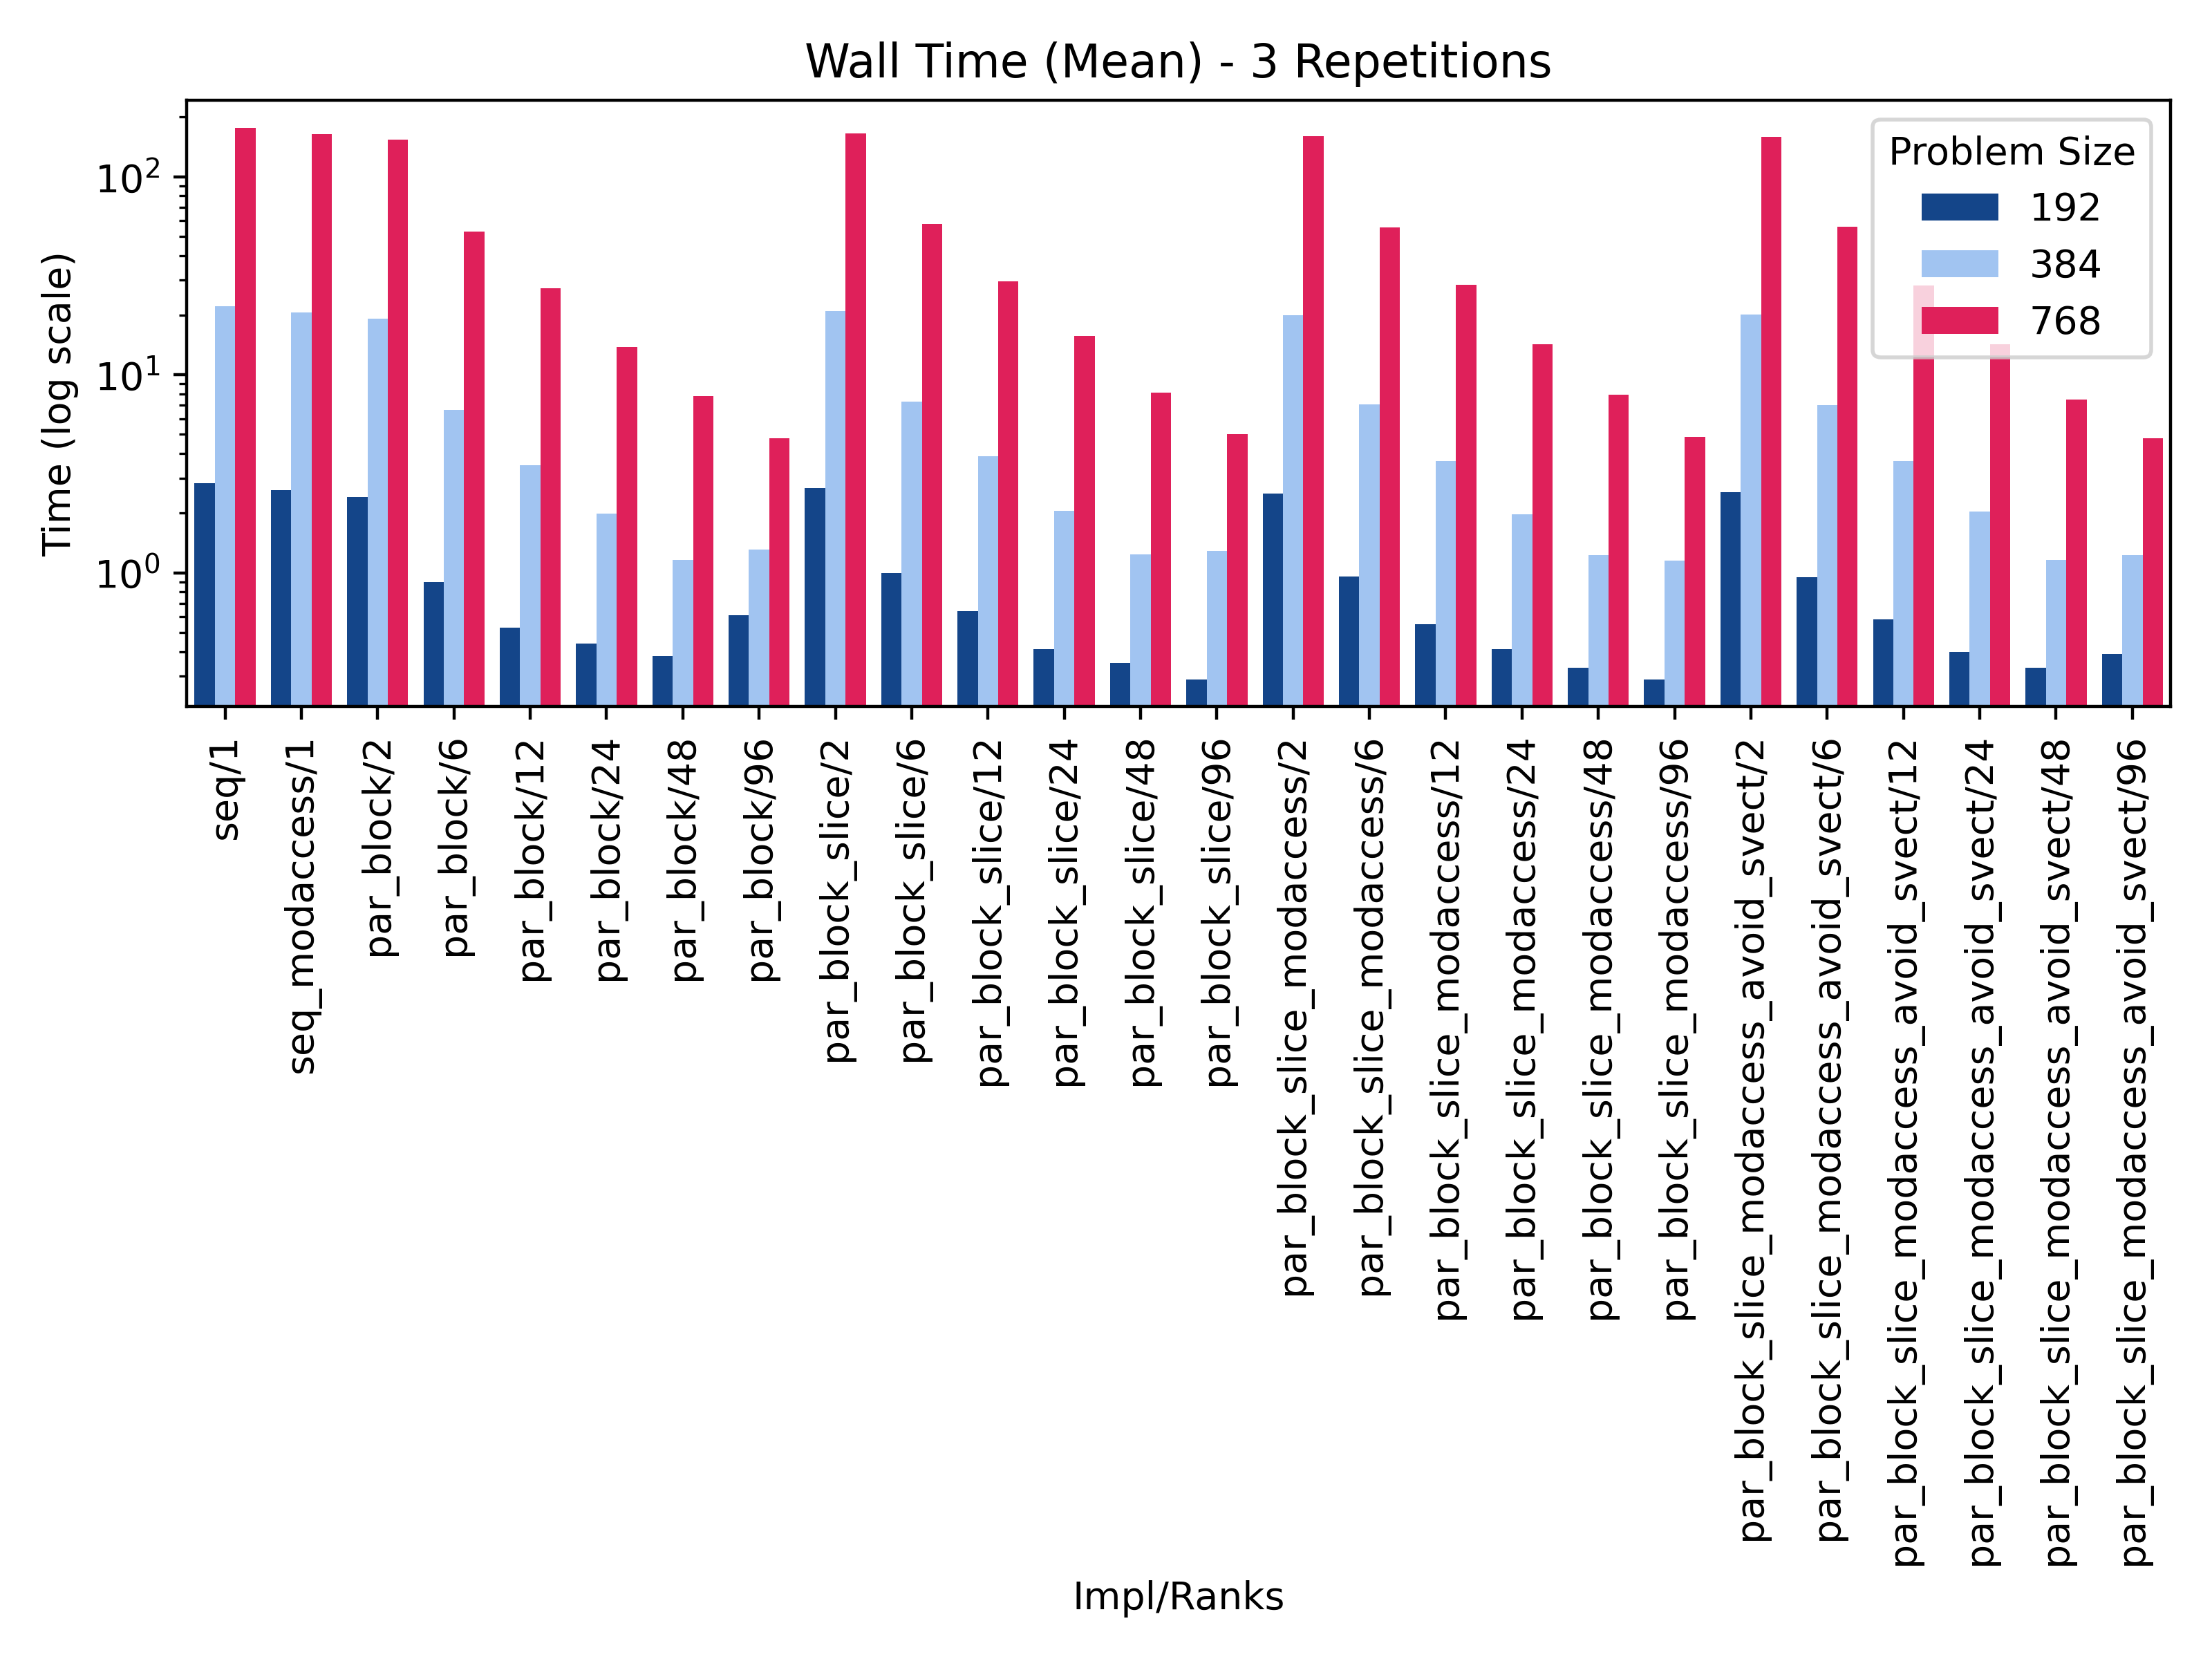
\includegraphics[width=0.9\linewidth]{images/measurements_wall_time}
	\caption{Wall time of all the different implementations.}
	\label{fig:measurementswalltime}
\end{figure}

\begin{figure}[H]
	\centering
	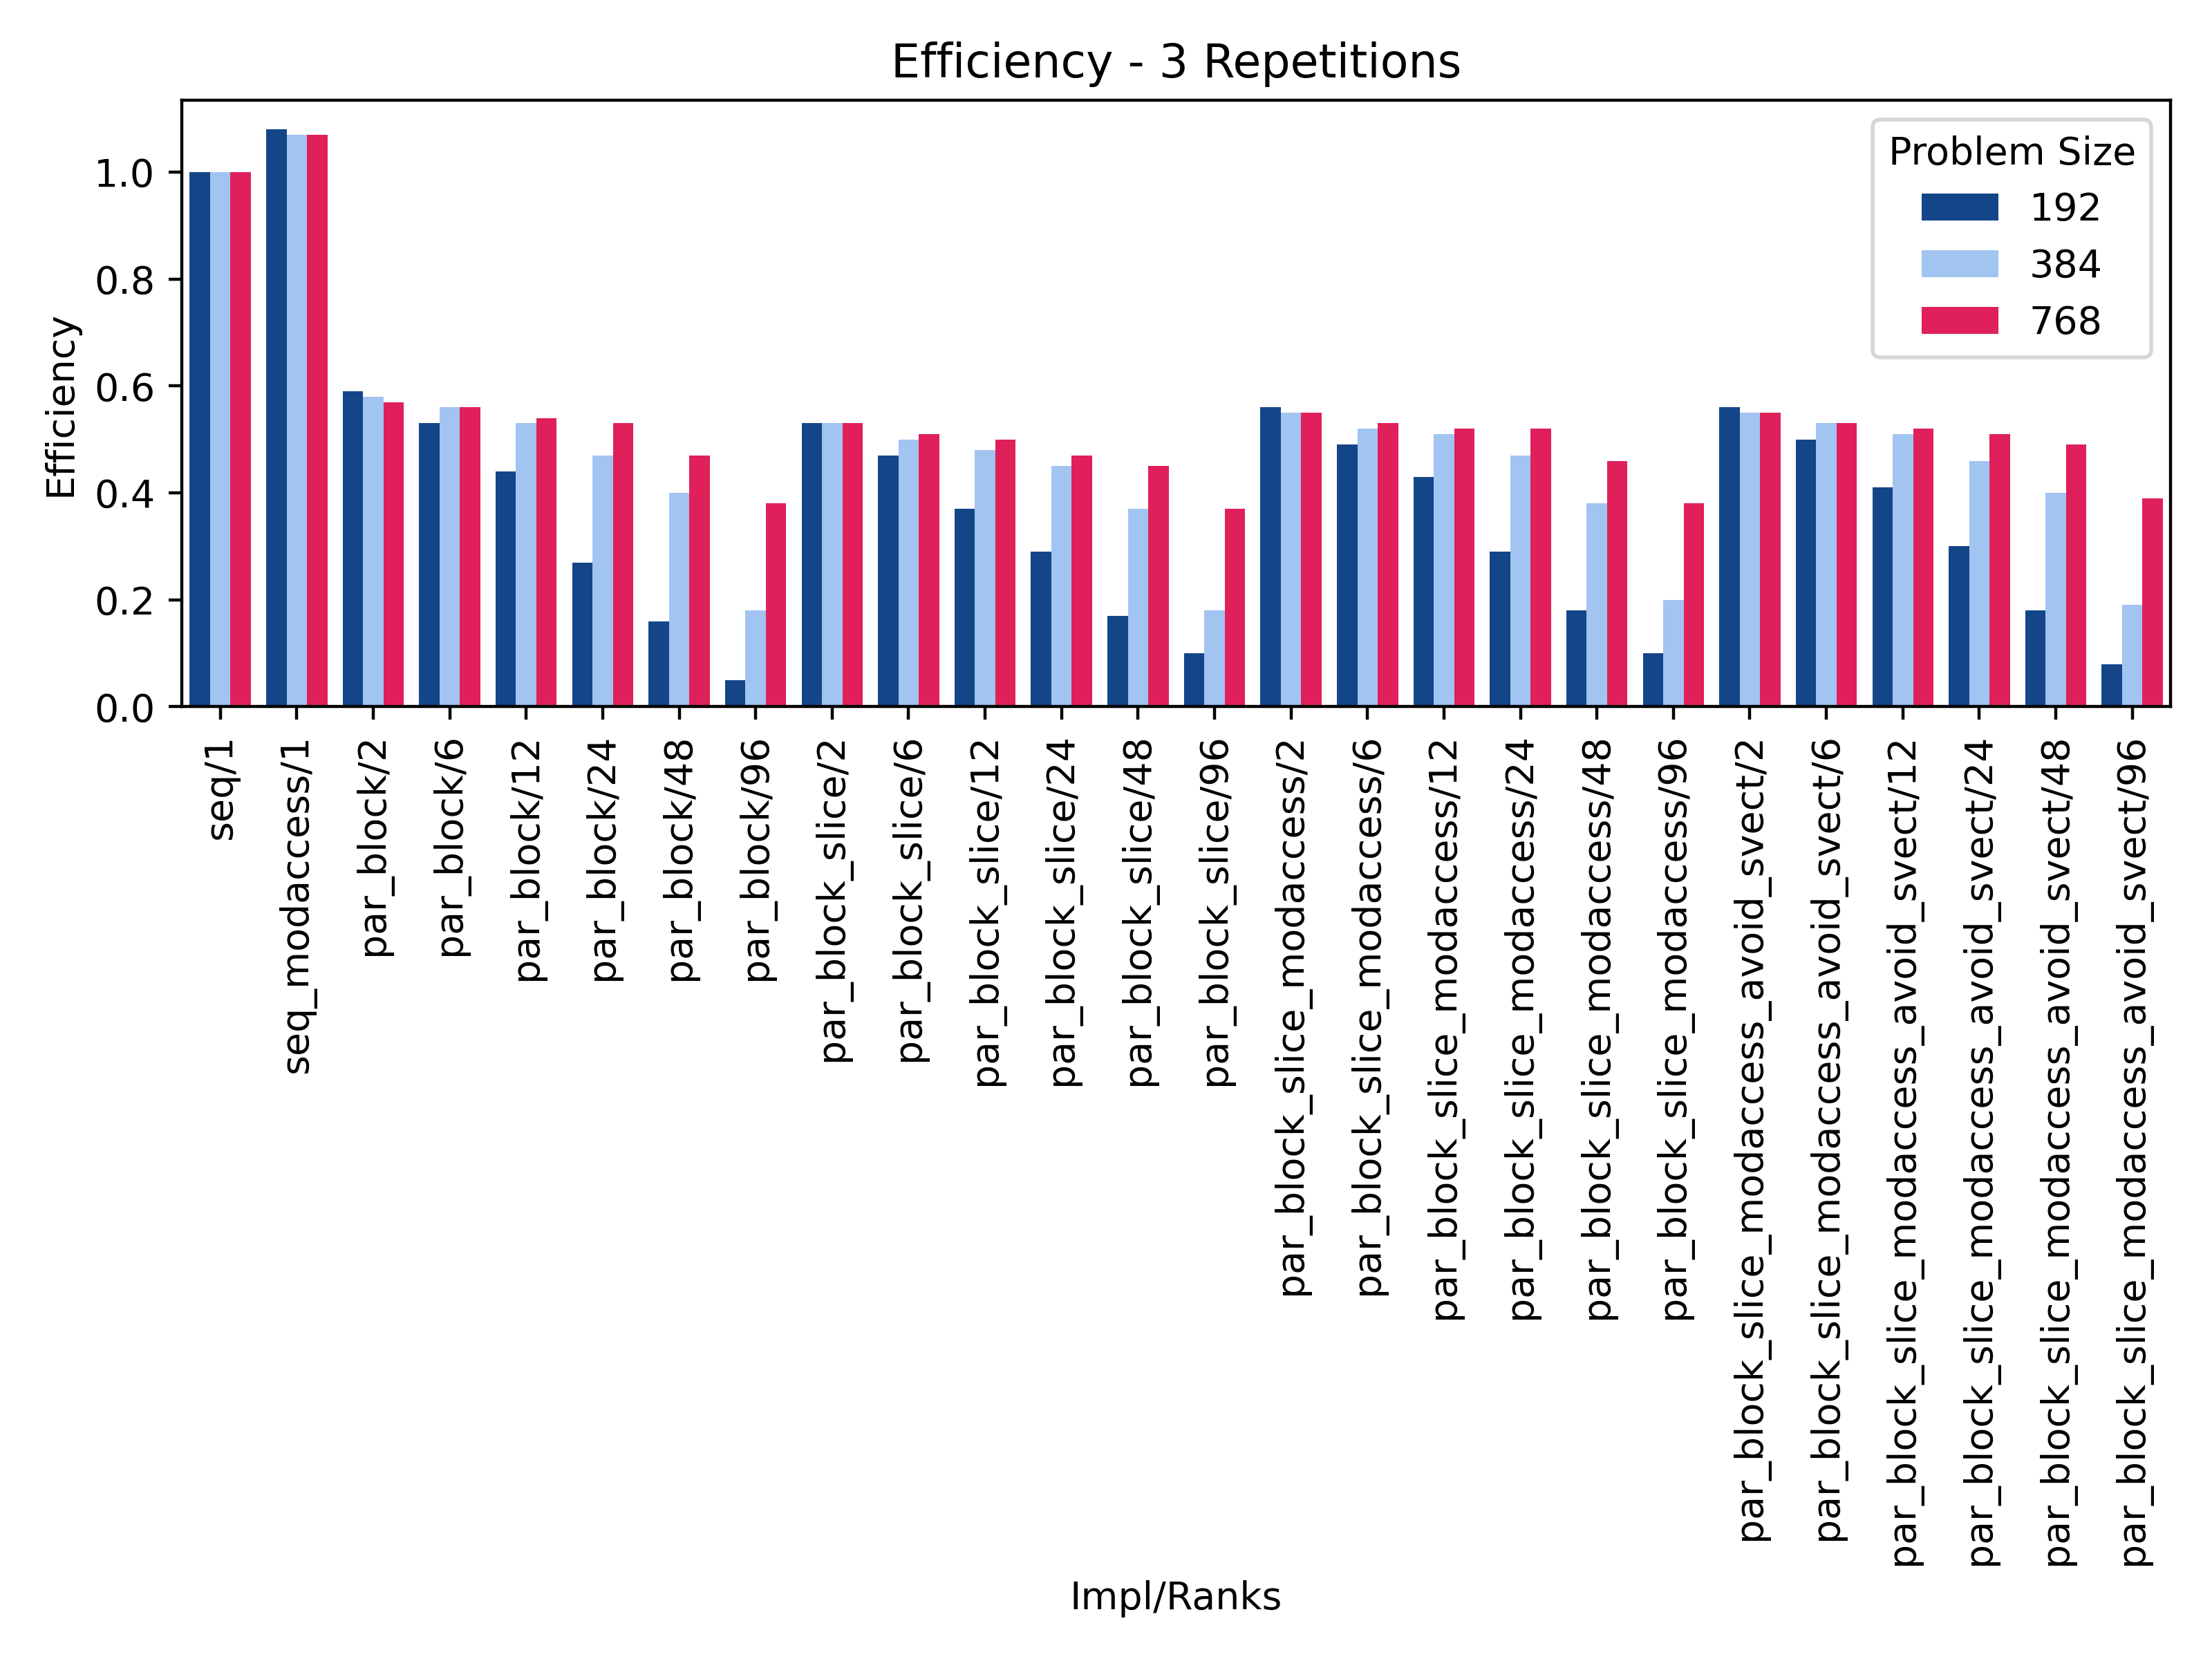
\includegraphics[width=0.9\linewidth]{images/measurements_efficiency.png}
	\caption{Efficiency of all the different implementations.}
	\label{fig:measurementsefficiency}
\end{figure}

\begin{figure}[H]
	\centering
	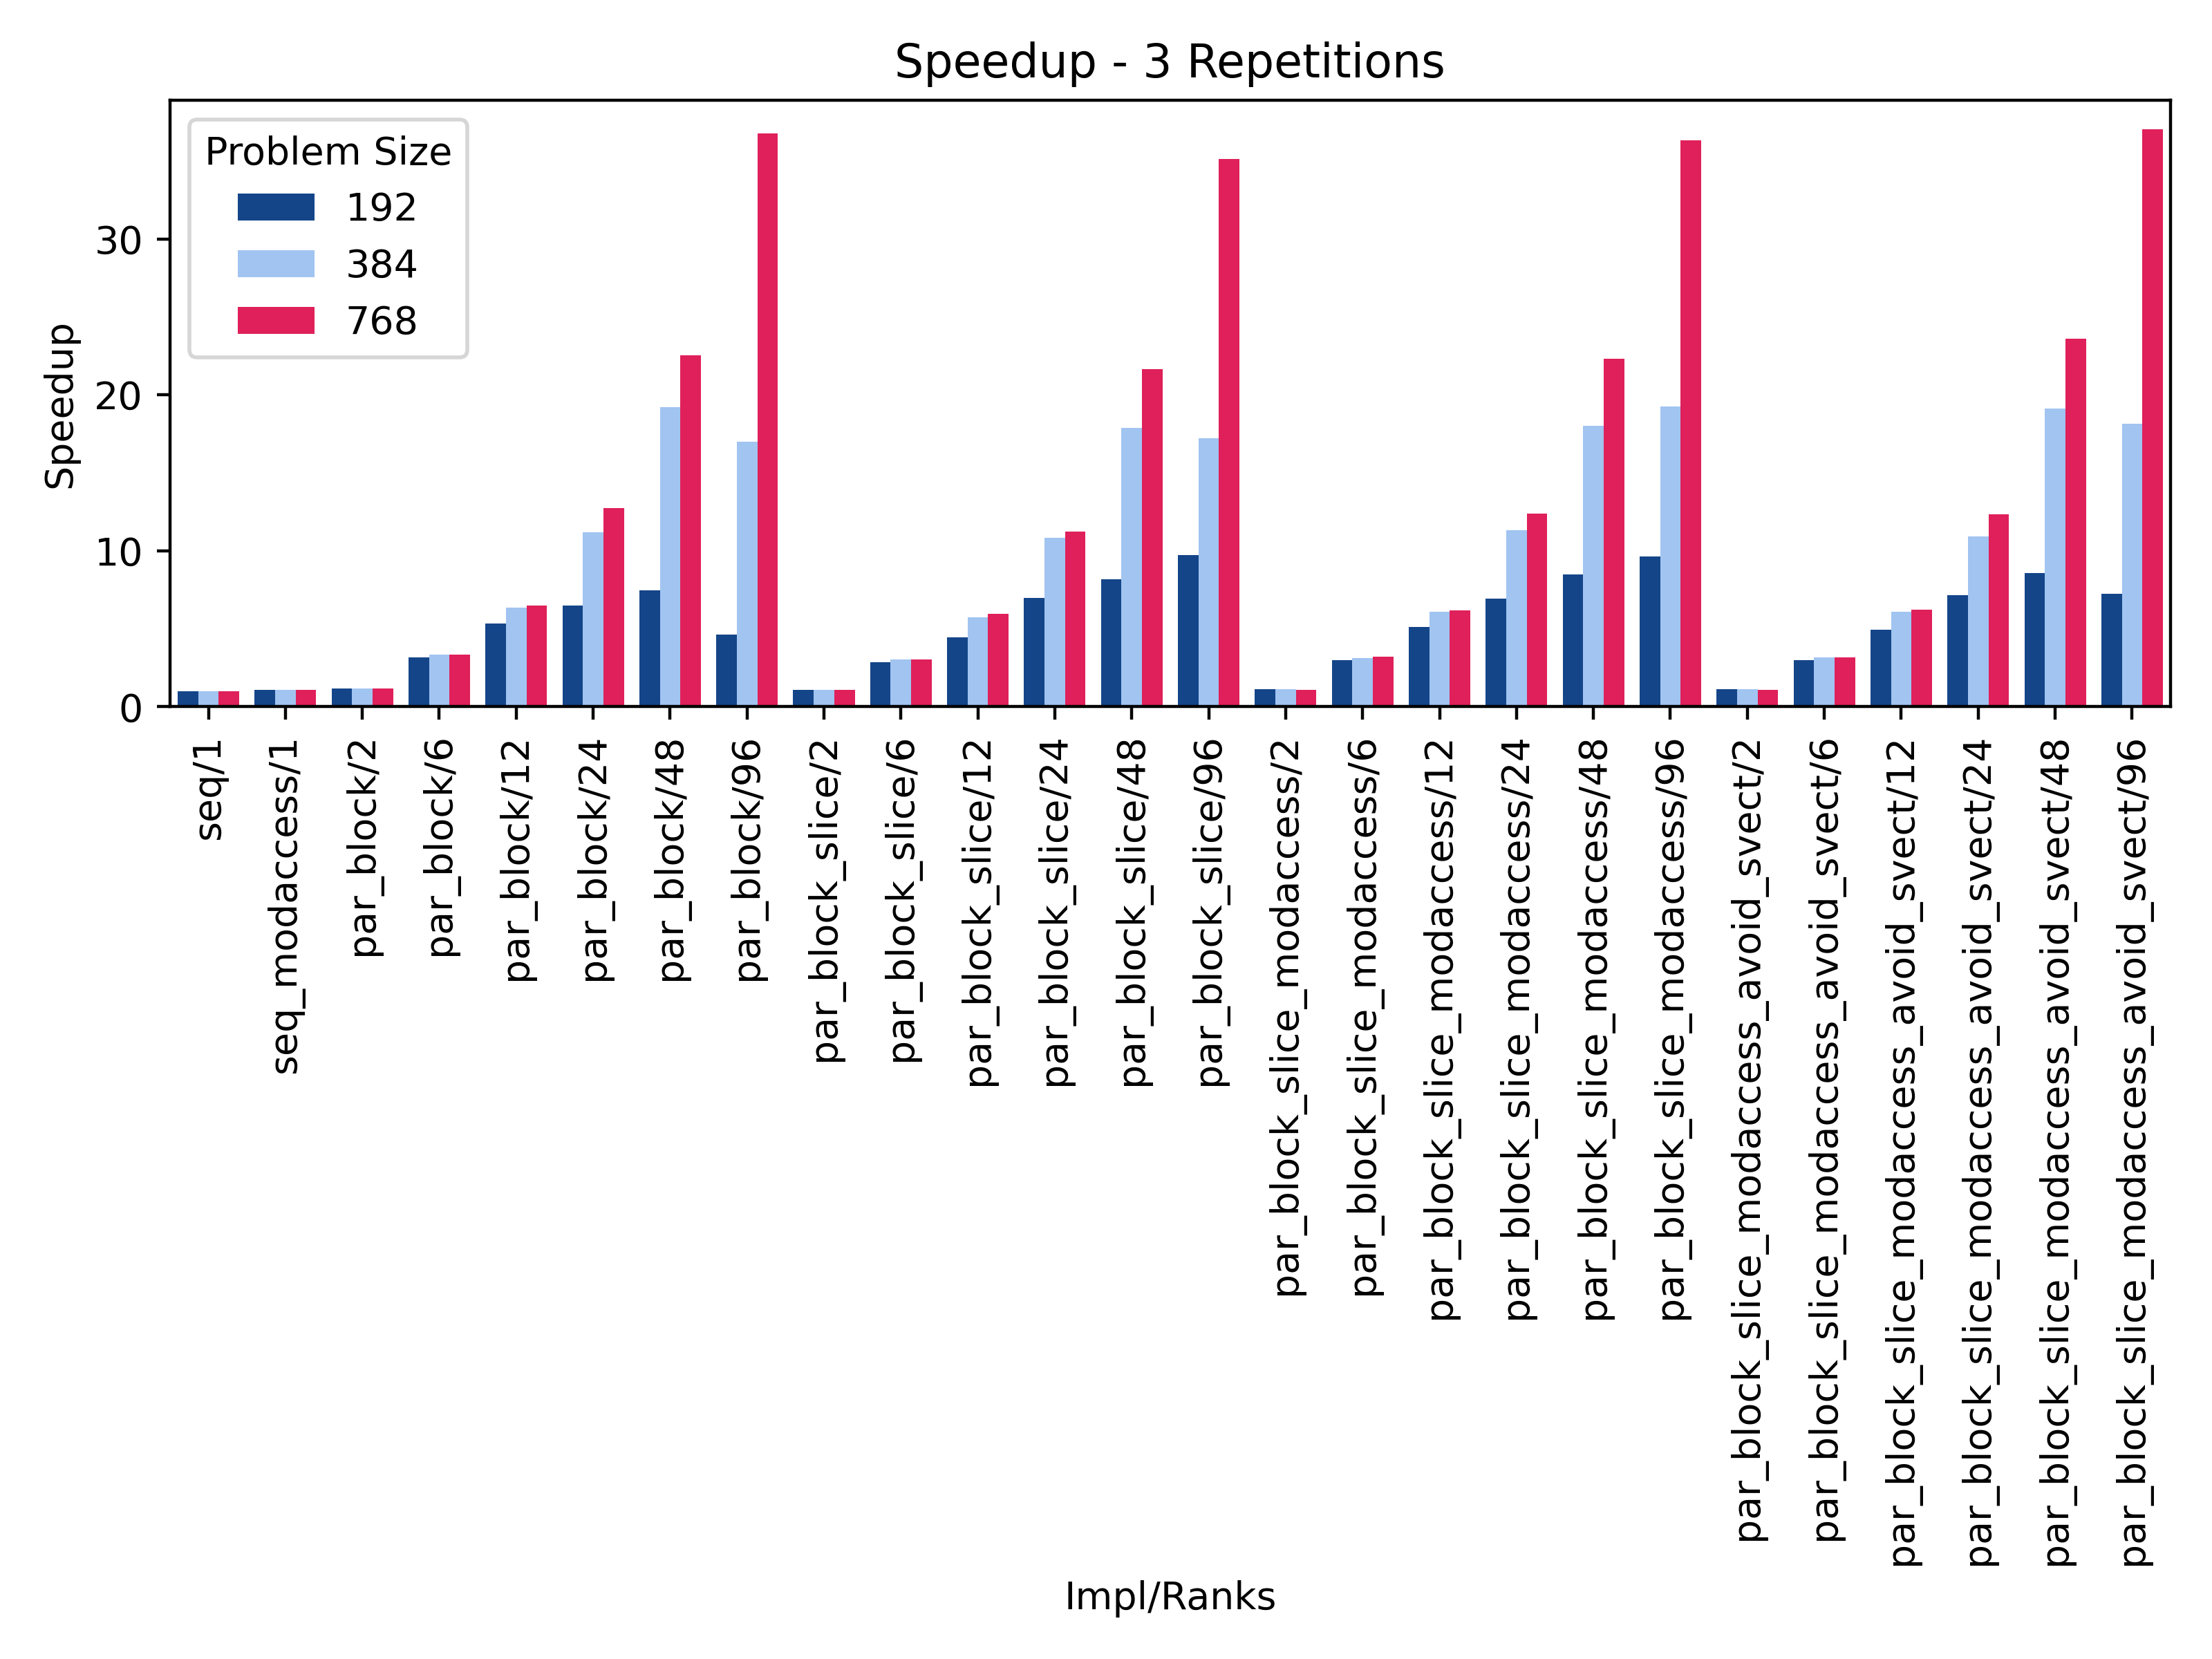
\includegraphics[width=0.9\linewidth]{images/measurements_speedup.png}
	\caption{Speedup of all the different implementations.}
	\label{fig:measurementsspeedup}
\end{figure}
    	
    	\begin{tabular}{|lllll|}
\hline
\multicolumn{5}{|c|}{\textbf{Results of 2D Heat Stencil Execution}} \\ \hline
\multicolumn{1}{|c|}{\textbf{Impl/Ranks}} & \multicolumn{4}{c|}{\textbf{Problem Size}} \\ \hline
\multicolumn{1}{|c|}{\textbf{}} & \multicolumn{4}{c|}{\textbf{384}} \\ \hline
\multicolumn{1}{|l|}{} & \multicolumn{1}{c|}{$\mu$ [s]} & \multicolumn{1}{c|}{$\sigma$ [s]} & \multicolumn{1}{c|}{S(p)} & \multicolumn{1}{c|}{E(p)} \\ \hline
\multicolumn{1}{|l|}{seq/1}  & \multicolumn{1}{r|}{54.70} & \multicolumn{1}{r|}{41.33} & \multicolumn{1}{r|}{1.00} & \multicolumn{1}{r|}{1.00}  \\ \hline
\multicolumn{1}{|l|}{par\_block/6}  & \multicolumn{1}{r|}{43.36} & \multicolumn{1}{r|}{49.53} & \multicolumn{1}{r|}{1.26} & \multicolumn{1}{r|}{0.21}  \\ \hline
\multicolumn{1}{|l|}{par\_non\_block/6}  & \multicolumn{1}{r|}{42.34} & \multicolumn{1}{r|}{49.14} & \multicolumn{1}{r|}{1.29} & \multicolumn{1}{r|}{0.22}  \\ \hline
\end{tabular}

    	
    	
    	
    	
    	
    	
    	
    	
    	
    	\item If you want to share your performance results of the improved version, insert the final walltime and speedup of the 2D stencil for 96 cores for N=768x768 and T=768x100 into the comparison spreadsheet: \href{https://docs.google.com/spreadsheets/d/1p6d9F12EtykmI2-7MnHkg0U15UAtaCvWz8Ip92ZEsWo}{spreadsheet}.
    \end{itemize}
    
    
    
\end{document}